Este capítulo tem a finalidade de apresentar como a pesquisa foi estruturada. Primeiramente, foram realizadas buscas por trabalhos que abordam a tecnologia blockchain, como estudos secundários e livros. Desta forma, obteve-se um panorama sobre os conceitos gerais envolvidos no funcionamento da blockchain, assim como características específicas que diferenciam blockchains distintas, em particular, a Bitcoin e a Ethereum. Assim, também foi observado em vários trabalhos que aplicações que executam sobre a blockchain Ethereum sofreram diversos ataques, especialmente devido à exploração de vulnerabilidades sobre os CIs, que foram um elemento crucial para a criação da Ethereum, bem como para sua popularização. Com base nisso, foi empregada uma estratégia para revisão bibliográfica conhecida como \sigla{MS}{Mapeamento Sistemático}, empregada neste trabalho com o objetivo de identificar e classificar o conteúdo relacionado à verificação para correção ou detecção de vulnerabilidades para aprimoramento da segurança dos CIs. O MS foi conduzido seguindo os métodos descritos por ~\citeonline{nakagawa2017revisao} e ~\citeonline{kitchenham2007guidelines}. Para descrever como foi conduzido o processo de pesquisa, tal como os métodos empregados, foram seguidas as seguintes tarefas:

\begin{enumerate}
    \item Planejamento e execução do MS;
    \item Seleção do método de verificação e detecção de vulnerabilidades adequado para a proposta;
    \item Seleção das vulnerabilidades abordadas por meio da proposta;
    \item Definição da estratégia para validação da proposta.
\end{enumerate}


\section{Mapeamento Sistemático} \label{tex:rev:ms}

%A etapa de MS tem o intuito de explorar a literatura sobre o tema verificação formal para correção ou detecção de vulnerabilidades para garantia de segurança de CIs.
O processo de MS empregado neste trabalho é realizado em três fases: (i) planejamento; (ii) condução; e (iii) publicação dos resultados. O planejamento do MS é a fase na qual é definido o objetivo e o protocolo do MS. No protocolo são especificados os procedimentos necessários para identificação dos estudos primários, tais como: questões de pesquisa; estratégia de busca; fontes de pesquisa; \textit{string} de busca; e critérios de seleção. A fase de condução consiste em identificar os estudos primários com base nas estratégias de busca e seleção, além de extrair e sintetizar os dados de forma a auxiliar o processo de resposta das questões de pesquisa. Por fim, na fase de publicação dos resultados, as questões de pesquisa são respondidas e os resultados são relatados e avaliados~\cite{nakagawa2017revisao, kitchenham2007guidelines}.  

Adiante, na Seção~\ref{tex:rev:ms:planejamento-cond}, são descritas as fases de planejamento e condução do MS, nas quais os itens relacionados ao protocolo do MS são retratados, os estudos primários são identificados e submetidos à extração de seus dados, e a estratégia de sintetização dos dados é definida. Em seguida, na Seção~\ref{tex:rev:ms:publicacao}, os resultados são obtidos e as questões de pesquisa respondidas. Por fim, na Seção~\ref{tex:rev:ms:discussao} há uma discussão acerta dos resultados obtidos.   

\subsection{Planejamento e condução}\label{tex:rev:ms:planejamento-cond}

O MS realizado neste trabalho tem o objetivo de revisar o estado da arte dos estudos realizados que abordam a verificação para correção ou detecção de vulnerabilidades para aprimoramento da segurança dos CIs, assim como classificar as abordagens empregadas e suas formas de implementação, identificar limitações existentes, e, por fim, analisar as estratégias de validação utilizadas.

Com o intuito de guiar o processo de revisão e satisfazer os objetivos, foram formuladas as questões de pesquisa. O foco das questões de pesquisas estão em identificar as abordagens utilizadas, assim como suas limitações e seus respectivos procedimentos de validação. Deste modo, baseado no objetivo deste MS, foram levantadas cinco questões de pesquisa (QP). São elas:

\begin{itemize}
    \item \textbf{QP 1.} Quais abordagens têm sido propostas?
    %\item \textbf{QP 2.} Quais ferramentas e frameworks foram desenvolvidos ou utilizados para aplicação das abordagens de verificação para correção ou detecção de vulnerabilidades para aprimoramento da segurança dos CIs?
    \item \textbf{QP 2.} Quando e onde os estudos têm sido aplicados?
    \item \textbf{QP 3.} Quais problemas ou vulnerabilidades relacionados aos CIs têm sido abordados?
    \item \textbf{QP 4.} Quais estratégias de validação foram utilizadas?
    \item \textbf{QP 5.} Quais são as limitações presentes nas abordagens?
\end{itemize}

Para levantamento dos estudos necessários para responder as questões de pesquisa, foram utilizados os motores de busca \textit{Engineering Village}~\footnote{\url{https://www.engineeringvillage.com/}}, \textit{Scopus}~\footnote{\url{https://www.scopus.com/}} e \textit{Web of Science}~\footnote{\url{https://www.webofknowledge.com}}. Como complemento, a pesquisa também foi realizada sobre as bases de dados bibliográficas \textit{IEEE Xplore}~\footnote{\url{https://ieeexplore.ieee.org/}} e \textit{ACM Digital Library}~\footnote{\url{https://dl.acm.org/}}. Todos os motores de busca e bases bibliográficas selecionados permitem especificar os campos sobre os quais a busca é executada. Neste MS, os repositórios foram configurados para efetuar a busca sobre o título, o resumo e as palavras-chave dos estudos. Além disso, no motor de busca \textit{Web of Science}, os resultados foram refinados para abranger apenas as categorias relacionadas à ciência da computação.

Com os repositórios de artigos definidos, o passo seguinte foi determinar a \textit{string} de busca, composta por palavras-chave e operadores lógicos para conduzir o processo de busca nos repositórios. Como exposto por ~\citeonline{nakagawa2017revisao}, o MS é um processo iterativo, pois, ao longo de seu desenvolvimento, pode-se notar a necessidade de ajustes no objetivo e no protocolo, que são então modificados, o protocolo é reavaliado, e o processo de condução recomeçado. Ao longo desta pesquisa, foram necessários alguns ajustes na \textit{string} de busca, a fim de adequar as palavras-chave escolhidas para abranger mais artigos relacionados com o objetivo deste MS. Por fim, obteve-se a seguinte \textit{string} de busca:

\begin{center}
    (\textit{``smart contract'' OR ``ethereum bytecode''}) \textit{AND} (\textit{verification OR validation OR monitor* OR analysis OR formalization OR ``formal methods'' OR ``security vulnerabilities'' OR ``security bugs'' OR ``vulnerability detection'' OR ``bug detection'' OR optimiz*})
\end{center}

% Please add the following required packages to your document preamble:
% \usepackage{multirow}
\begin{table}[!ht]
\centering
\caption{Quantidade de estudos encontrados nos repositórios}
\label{tab:rev:repositorios}
\begin{tabular}{|l|c|}
\hline
\textbf{Repositórios}                & \textbf{Nº de estudos} \\ \hline
Engineering Village                  & 865                    \\ \hline
Scopus                               & 906                    \\ \hline
Web of Science                       & 170                    \\ \hline
ACM Digital Library                  & 65                     \\ \hline
IEEE Xplore                          & 85                     \\ \hline
\multicolumn{1}{|r|}{\textbf{Total}} & \textbf{2091}          \\ \hline
\end{tabular}
\fdadospesquisa
\end{table}
% \FloatBarrier

Uma vez definida a \textit{string} de busca, as buscas nos repositórios foram realizadas. Considerando a eliminação de artigos duplicados, a quantidade de estudos encontrados em cada repositório é apresentada na Tabela~\ref{tab:rev:repositorios}. O levantamento dos trabalho ocorreu semanalmente, assim, o mecanismo de busca das bases bibliográficas e dos motores de busca foram configurados para enviarem atualizações semanais.

Após o levantamento dos artigos, foram aplicadas duas fases de revisão para selecionar apenas os trabalhos relevantes para esta pesquisa. Na primeira fase, a revisão inicial, o resumo de cada artigo foi lido, e, quando necessário, a introdução e a conclusão também, e então cada trabalho foi incluído ou excluído da revisão de acordo com critérios de seleção predefinidos. Em caso de dúvida, o estudo foi aceito na revisão inicial para ser novamente analisado na fase seguinte. Assim, obteve-se o conjunto provisório de estudos primários aceitos, sobre o qual foi realizada a fase de revisão final. Nesta fase, cada artigo teve todo seu texto lido, e então foi novamente submetido aos critérios de seleção. O processo de planejamento e condução deste MS é ilustrado na Figura~\ref{fig:ms_fluxo}.

\begin{figure}[!ht]
 \caption{Fluxo de atividades das fases de planejamento e condução do MS}
 \label{fig:ms_fluxo}
 \centering
 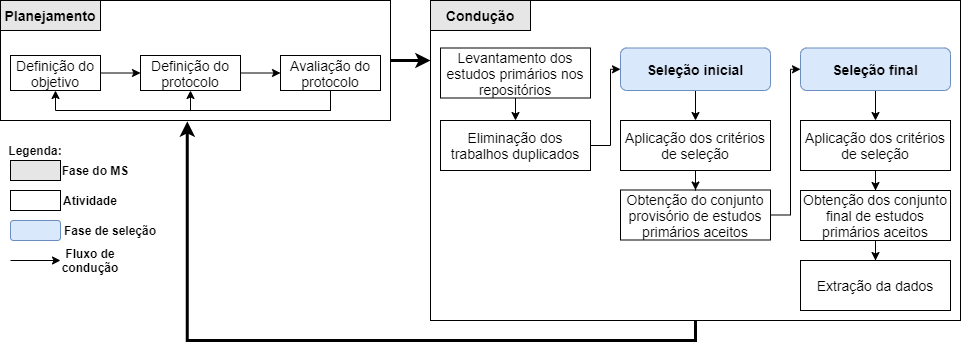
\includegraphics[scale=0.5]{figuras/ms_fluxo.png}
 \fautor
\end{figure}

Para selecionar os estudos relacionados ao tópico de pesquisa deste MS, foi definido o seguinte critério de inclusão (CrI):

\begin{itemize}
    \item \textbf{CrI 1.} O estudo propõe uma abordagem que é utilizada para verificação formal para correção ou detecção de vulnerabilidades para garantia de segurança de CIs?
\end{itemize}

Os estudos excluídos foram rejeitados de acordo com sua adequação à pelo menos um dos seguintes critérios de exclusão (CE): 

\begin{itemize}
    \item \textbf{CE 1.} O estudo não propõe uma abordagem que é utilizada para verificação formal para correção ou detecção de vulnerabilidades para garantia de segurança de CIs?
    \item \textbf{CE 2.} O estudo não possui o texto completo publicado?
    \item \textbf{CE 3.} O estudo não é escrito na língua inglesa?
    \item \textbf{CE 4.} O estudo é uma versão antiga de outro artigo selecionado?
    \item \textbf{CE 5.} O estudo não é um estudo primário?
    \item \textbf{CE 6.} Não foi possível acessar o texto completo do estudo?
\end{itemize}

Depois da eliminação dos estudos duplicados e da execução das fases de seleção inicial e final, obteve-se os estudos primários necessários para responder às questões de pesquisa. A quantidade de estudos aceitos e rejeitados de cada repositório é exposta na Tabela~\ref{tab:rev:selecao-final}, somando um total de 104 estudos selecionados. Na Tabela~\ref{tab:rev:estudos-selecionados} é listada a citação e o identificador ($#ID$) de cada estudo selecionado. No decorrer deste capítulo, os identificadores são utilizados para se referir à publicação correspondente. 

\begin{table}[!ht]
\centering
\caption{Quantidade de estudos primários selecionados em cada repositório}
\label{tab:rev:selecao-final}
\begin{tabular}{|l|c|c|}
\hline
\textbf{Repositórios} & \textbf{Aceitos} & \textbf{Rejeitados} \\ \hline
Engineering Village & 41 & 824 \\ \hline
Scopus  & 47 & 859 \\ \hline
Web of Science & 5 & 165 \\ \hline
ACM Digital Library & 7 & 58 \\ \hline
IEEE Xplore & 4 & 81 \\ \hline
\multicolumn{1}{|r|}{\textbf{Total}} & \textbf{104} & \textbf{1987} \\ \hline
\end{tabular}
\fdadospesquisa
\end{table}
%\FloatBarrier

\begin{table}[!ht]
\centering
\fontsize{8pt}{8pt}\selectfont
\addtolength{\tabcolsep}{-4pt}
\caption{Estudos selecionados}
\label{tab:rev:estudos-selecionados}
\begin{tabular}{@{}llllll@{}}
\toprule
\multicolumn{1}{l}{\textbf{ID}} &
  \multicolumn{1}{l}{\textbf{Citação}} &
  \multicolumn{1}{l}{\textbf{ID}} &
  \multicolumn{1}{l}{\textbf{Citação}} &
  \multicolumn{1}{l}{\textbf{ID}} &
  \multicolumn{1}{l}{\textbf{Citação}} \\ \midrule
\#01  &  \citeonline{ferreira2020aegis-01} & \#36 & \citeonline{prechtel2019evaluating-36} & \#71  & \citeonline{li2020research-71} \\
\#02  & \citeonline{fu2019critical-02} & \#37 & \citeonline{kolluri2019exploiting-37} & \#72  & \citeonline{li2020safepay-72} \\
\#03  & \citeonline{sun2020formal-03} & \#38 & \citeonline{yang2019fether-38} & \#73  & \citeonline{albert2019safevm-73} \\
\#04  & \citeonline{wang2020formal-04} & \#39 & \citeonline{nikolic2018finding-39} & \#74  & \citeonline{chang2019scompile-74} \\
\#05  & \citeonline{park2018formal-05} & \#40 & \citeonline{duo2020formal-40}  & \#75  & \citeonline{hao2020scscan-75} \\
\#06  & \citeonline{du2020general-06} & \#41 & \citeonline{bai2018formal-41} & \#76  & \citeonline{tsankov2018securify-76} \\
\#07  & \citeonline{yang2020hybrid-07} & \#42 & \citeonline{liu2019formal-42} & \#77  & \citeonline{li2020securing-77} \\
\#08  & \citeonline{xing2020new-08} & \#43 & \citeonline{li2019formal-43} & \#78  & \citeonline{kongmanee2019securing-78} \\
\#09  & \citeonline{da2020tool-09} & \#44 & \citeonline{abdellatif2018formal-44} & \#79  & \citeonline{zhou2018security-79} \\
\#10 & \citeonline{marescotti2020accurate-10} & \#45 & \citeonline{qu2018formal-45} & \#80  & \citeonline{peng2019sif-80} \\
\#11 & \citeonline{lahbib2020event-11} & \#46 & \citeonline{madl2019formal-46} & \#81  & \citeonline{feist2019slither-81} \\
\#12 & \citeonline{weiss2019annotary-12} & \#47 & \citeonline{bhargavan2016formal-47} & \#82  & \citeonline{tian2019smart-82} \\
\#13 & \citeonline{wang2020artemis-13} & \#48 & \citeonline{wang2019formal-48} & \#83  & \citeonline{yu2020smart-83} \\
\#14 & \citeonline{sun2021attention-14} & \#49 & \citeonline{ding2020function-49} & \#84  & \citeonline{zhuangsmart-84} \\
\#15 & \citeonline{beillahi2020behavioral-15} & \#50 & \citeonline{chen2020gaschecker-50} & \#85  & \citeonline{tikhomirov2018smartcheck-85} \\
\#16 & \citeonline{gao2020checking-16} & \#51 & \citeonline{ashraf2020gasfuzzer-51} & \#86  & \citeonline{zhang2020smartshield-86} \\
\#17 & \citeonline{marescotti2018computing-17} & \#52 & \citeonline{wustholz2020harvey-52} & \#87  & \citeonline{alt2018smt-87} \\
\#18 & \citeonline{jiang2018contractfuzzer-18} & \#53 & \citeonline{huang2021hunting-53} & \#88  & \citeonline{akca2019solanalyser-88} \\
\#19 & \citeonline{wang2019contractguard-19} & \#54 & \citeonline{momeni2019machine-54} & \#89  & \citeonline{hajdu2019solc-89} \\
\#20 & \citeonline{wang2020contractward-20} & \#55 & \citeonline{grech2018madmax-55} & \#90  & \citeonline{liao2019soliaudit-90} \\
\#21 & \citeonline{xue2020cross-21} & \#56 & \citeonline{luu2016making-oyente-56} & \#91  & \citeonline{lai2020static-91} \\
\#22 & \citeonline{shishkin2019debugging-22} & \#57 & \citeonline{mossberg2019manticore-57} & \#92  & \citeonline{feng2020summary-92} \\
\#23 & \citeonline{nehai2019deductive-23} & \#58 & \citeonline{osterland2020model-58} & \#93  & \citeonline{krupp2018teether-93} \\
\#24 & \citeonline{hirai2017defining-24} & \#59 & \citeonline{nehai2018model-59} & \#94  & \citeonline{torres2019art-94} \\
\#25 & \citeonline{ji2020deposafe-25} & \#60 & \citeonline{he2020modeling-60} & \#95  & \citeonline{mavridou2018tool-95} \\
\#26 & \citeonline{wang2019detecting-nondeterministic-26} & \#61 & \citeonline{azzopardi2018monitoring-61} & \#96  & \citeonline{qian2020towards-96} \\
\#27 & \citeonline{arganaraz2020detection-27} & \#62 & \citeonline{zhang2019mpro-62} & \#97  & \citeonline{liu2020towards-97} \\
\#28 & \citeonline{atzei2019developing-28} & \#63 & \citeonline{lu2019neucheck-63} & \#98  & \citeonline{chen2018towards-98} \\
\#29 & \citeonline{albert2021don-29} & \#64 & \citeonline{wang2020oracle-64} & \#99  & \citeonline{amani2018towards-99} \\
\#30 & \citeonline{gao2019easyflow-30} & \#65 & \citeonline{torres2018osiris-65} & \#100 & \citeonline{ahrendt2019verification-100} \\
\#31 & \citeonline{brent2020ethainter-31} & \#66 & \citeonline{yamashita2019potential-66} & \#101 & \citeonline{nelaturu2020verified-101} \\
\#32 & \citeonline{frank2020ethbmc-32} & \#67 & \citeonline{chatterjee2018quantitative-67} & \#102 & \citeonline{so2020verismart-102}  \\
\#33 & \citeonline{ashouri2020etherolic-33} & \#68 & \citeonline{chinen2020ra-68} & \#103 & \citeonline{mavridou2019verisolid-103} \\
\#34 & \citeonline{schneidewind2020ethor-34} & \#69 & \citeonline{samreen2020reentrancy-69} & \#104 & \citeonline{permenev2020verx-104} \\
\#35 & \citeonline{zhang2020ethploit-35} & \#70 & \citeonline{liu2018reguard-70} &       &  \\ \bottomrule
\end{tabular}
\fdadospesquisa
\end{table}

A partir do conjunto final de estudos primários aceitos, foi feita a extração de dados desses trabalhos, na qual informações foram coletadas com o intuito de auxiliar na resposta das questões de pesquisa.

Para condução de um MS, é preciso determinar um esquema de classificação para guiar a extração e sintetização dos dados~\cite{petersen2008systematic}. Para as questões de pesquisa \textbf{QP 1}, \textbf{QP 3} e \textbf{QP 4} a estratégia de classificação foi definida levando em consideração informações coletadas dos próprios estudos selecionados. Para a \textbf{QP 2} não foi necessário determinar um esquema de classificação, já que trata apenas de informações como o ano e o veículo de publicação dos estudos. Para a \textbf{QP 4} alguns aspectos dos estudos foram analisados, mas nem todos possuem uma classificação direta, já que alguns dados foram coletados de forma não estruturada e sem uma classificação predefinida. As categorias e classificações definidas são expostas a seguir. 

\subsubsection*{Abordagens propostas (\textbf{QP 1})}

Diversas técnicas foram propostas para verificação e correção de CIs com o intuito de mitigar problemas de segurança e a exposição à ataques que visam a exploração de vulnerabilidades no códigos dos contratos para obtenção de benefícios. A partir dos estudos selecionados, foram consideradas dez categorias. São elas: Análise estática; análise dinâmica; análise simbólica; execução simbólica; demonstração de teoremas; \textit{model checking}; verificação dedutiva; \textit{fuzzing}; IA; e Outras. 

Nos trabalhos selecionados, observou-se quatro variações das abordagens baseadas em \textit{model checking}, como o \textit{model checking} tradicional, o simbólico, o limitado, e o estatístico. Entre as abordagens que utilizam IA, duas técnicas específicas são utilizadas: \textit{machine learning}; e \textit{deep learning}. As variações das abordagens de \textit{model checking} e IA são consideradas como sub-categorias e são tratadas separadamente nos resultados da \textit{QP 1}. Já as técnicas observadas em apenas um dos estudos selecionados são englobadas na categoria Outras.

As abordagens também são classificadas de acordo com o tipo de verificação, sendo que, neste MS, foram identificados dois tipos: proativa; e em tempo de execução. 

\subsubsection*{Ano e veículo de publicação dos estudos (\textbf{QP 2})}

Para responder esta questão de pesquisa, foi contabilizada a quantidade de estudos publicados em cada ano. Para cada ano, também foi observado quantos estudos se enquadram em cada uma das abordagens para verificação definidas na \textbf{QP 1}. Ademais, os veículos de publicação foram classificados como Conferências, Periódicos e Workshops.

\subsubsection*{Problemas e vulnerabilidades abordados (\textbf{QP 3})}

Os estudos realizados para verificação de CIs têm como foco diversas vulnerabilidades e problemas para serem verificados. Além da detecção de vulnerabilidades específicas, várias abordagens permitem a detecção de violação de propriedades específicas para cada contrato, que podem ser propriedades funcionais, lógicas, ou baseadas nos requerimentos e requisitos de cada CI. Neste MS, a violação de propriedades é definida com uma categoria de problemas e vulnerabilidades abordadas. Ademais, algumas abordagens têm foco na correção sintática e semântica dos CIs, o que define mais uma categoria a ser analisada. As vulnerabilidades de segurança tratadas pelos estudos são classificadas em 23 tipos. Na Tabela~\ref{tab:rq3-vulnerabilidades} são listadas todas as vulnerabilidades e problemas considerados para responder esta questão de pesquisa, cada um acompanhado da respectiva sigla.

\subsubsection*{Estratégias de validação (\textbf{QP 4})}

De forma geral, nas pesquisas desenvolvidas para verificação de CIs, alguma ferramenta ou framework é implementado para validação do método proposto, ou é utilizado algum já existente. Em alguns casos, o método proposto não é implementado, e sua aplicação é descrita apenas como um processo. Em todos os casos, alguma estratégia é utilizada para validação da proposta. Baseado nos estudos selecionados, os mecanismos de aplicação das propostas (\textit{M}) são definidos conforme segue:
\begin{itemize}
    \item \textit{M1.} Implementação de um framework ou ferramenta;
    \item \textit{M2.} Utilização de um framework ou ferramenta já existente;
    \item \textit{M3}. Descrição de um processo.
\end{itemize}

As estratégias de validação das propostas são classificadas em três categorias, definidas com base nos estudos selecionados. São elas:
\begin{itemize}
    \item \textbf{Experimento:} A avaliação da proposta é feita a partir da definição de métricas como acurácia, eficiência, custo, performance, entre outras. O processo de experimentação dos métodos de verificação de CIs englobam ao menos um dos seguintes procedimentos: (i) experimento em larga escala, no qual é obtida uma amostra grande, geralmente com milhares de CIs com vulnerabilidades previamente conhecidas ou não; (ii) experimento reduzido, em que é utilizada uma amostra relativamente pequena de CIs, que pode variar de algumas unidades até centenas de contratos, geralmente com vulnerabilidades previamente conhecidas. Em alguns casos, essa amostra de contratos é obtida a partir de critérios predefinidos, formando um \textit{benchmark} de CIs; (iii) avaliação empírica, na qual uma ou mais ferramentas, frameworks ou técnicas conhecidas na literatura são utilizados no experimento para comparação dos resultados e comprovação de avanços e melhorias;
    \item \textbf{Estudo de caso:} Como prova de conceito, um ou mais CIs previamente conhecidos são analisados e verificados por meio do método proposto. Na sequência, os resultados são examinados, e a aplicabilidade da proposta é esclarecida;  
    \item \textbf{Exemplo de aplicação:} Como prova de conceito, são descritos um ou mais exemplos simples de utilização da proposta.  
\end{itemize}

\subsubsection*{\textbf{Limitações (QP 5)}}

A verificação e detecção de vulnerabilidades em CIs é uma área de pesquisa recente, e, como relatado por ~\citeonline{chen2020survey-ethereum-acm} e ~\citeonline{kim2020automated-test-sc}, as abordagens existentes apresentam diversas limitações. Para responder esta questão de pesquisa, dois aspectos foram considerados para classificação sistemática dos estudos. São eles:

\begin{itemize}
    \item \textbf{Abrangência limitada}: A verificação não abrange todos os elementos dos CIs, mas apenas algum sub-conjunto da linguagem Solidity;
    \item \textbf{Nível de automação}: Mesmo que a estratégia proposta execute a verificação de forma automática, alguns trabalhos manuais podem ser necessários, como tradução de código, obtenção do modelo do contrato, especificação de propriedades, e a análise e interpretação dos resultados.
\end{itemize}

Outros dois aspectos que foram aspectos observados, mas que não são classificados de forma sistemática, são:

\begin{itemize}
    \item \textbf{Necessidade de conhecimento prévio}: Para aplicação da abordagem é necessário ter o domínio de alguma linguagem ou formalismo específico para modelagem do contrato ou para definição dos padrões de vulnerabilidades e propriedades a serem verificadas;
    \item \textbf{Acurácia}: A ferramenta ou framework proposto para detecção de vulnerabilidades de CIs retornar falsos positivos e falsos negativos entre seus resultados.
\end{itemize}

Dentre os aspectos analisados para definir as limitações das abordagens de verificação, os dados sobre a abrangência limitada e o nível de automação foram coletados de forma estruturada sobre todos os estudos. Para as demais limitações, não foi estabelecida uma classificação predefinida, pois estas podem variar de acordo com a abordagem empregada e não seguem um padrão que permita uma classificação sistemática dos estudos.

\begin{table}[!ht]
\centering
\fontsize{8pt}{8pt}\selectfont
\caption{Vulnerabilidades e problemas alvos de verificação em CIs}
\label{tab:rq3-vulnerabilidades}
\begin{tabular}{@{}llll@{}}
\toprule
\textbf{Sigla} & \textbf{Vulnerabilidade / Problema} & \textbf{Sigla} & \textbf{Vulnerabilidade / Problema} \\ \midrule
$V_{1}$  & Ataque de profundidade da pilha de chamadas & $V_{14}$ & Dependência de \textit{timestamp}       \\
$V_{2}$  & Ataque DoS com operações ilimitadas         & $V_{15}$ & Desordem de exceções           \\
$V_{3}$  & Autenticação com \textit{tx.origin}                  & $V_{16}$ & Divisão por zero               \\
$V_{4}$  & Bloqueio de Ether                           & $V_{17}$ & Endereço curto                 \\
$V_{5}$  & Consumo de \textit{gas} ineficiente                  & $V_{18}$ & Exceções não tratadas          \\
$V_{6}$  & Contrato guloso                             & $V_{19}$ & Chamada externa não verificada \\
$V_{7}$  & Contrato pródigo                            & $V_{20}$ & \textit{Integer overflow} e \textit{underflow}   \\
$V_{8}$  & Contrato suicida                            & $V_{21}$ & Gasto de \textit{gas} descontrolado     \\
$V_{9}$  & Contrato \textit{honeypot}                           & $V_{22}$ & Problemas de concorrência      \\
$V_{10}$ & Controle de acesso vulnerável               & $V_{23}$ & Reentrância                    \\
$V_{11}$ & \textit{Delegatecall injection}             & $VP$  & Violação de propriedades       \\
$V_{12}$ & Dependência de informação do bloco          & $CSS$ & Correção sintática e semântica \\
$V_{13}$ & Dependência de ordem da transação           &       &                                \\ \bottomrule
\end{tabular}
\end{table}

%-------------------------------------------------------%
\subsection{Resultados}\label{tex:rev:ms:publicacao}

O MS foi executado de acordo com os passos descritos na Seção~\ref{tex:rev:ms:planejamento-cond}. Nesta seção são apresentados os resultados para cada questão de pesquisa. Para isso, foi utilizado um formulário de extração de dados com o ID do estudo, dados bibliográficos e informações referentes às classificações utilizadas. Tais dados e informações foram utilizados para extrair as respostas das questões de pesquisa, e, posteriormente, para exibição dos resultados.

\subsubsection*{\textbf{Abordagens para verificação de CIs (QP 1)}}

% execução simbólica é um tipo de abordagem dinâmica, mas foi tratada separadamente devido ao número expressivo de trabalhos encontrado que usam essa técnica específica e também por conta de sua peculiaridade de utilizar SMT solvers para verificação

Em 93 dos trabalhos selecionados é utilizada apenas uma das abordagens categorizadas nesta questão de pesquisa, com exceção de 11 trabalhos, que utilizam abordagens híbridas, nas quais duas técnicas são utilizadas em conjunto. Com o intuito de expor as principais abordagens mais utilizadas para verificação para correção e aprimoramento da segurança de CIs, no gráfico da Figura~\ref{fig:rq1-abordagens} é apontado o número de estudos em que cada abordagem foi empregada dentre 104 selecionados, na qual pode-se observar uma prevalência das técnicas de execução simbólica, \textit{model checking} e análise estática. Na tabela~\ref{tab:rq1-hibridas} são mostrados os estudos que empregaram abordagens híbridas.

\begin{figure}[!htb]
 \caption{Abordagens para verificação de CIs utilizadas}
 \label{fig:rq1-abordagens}
 \centering
 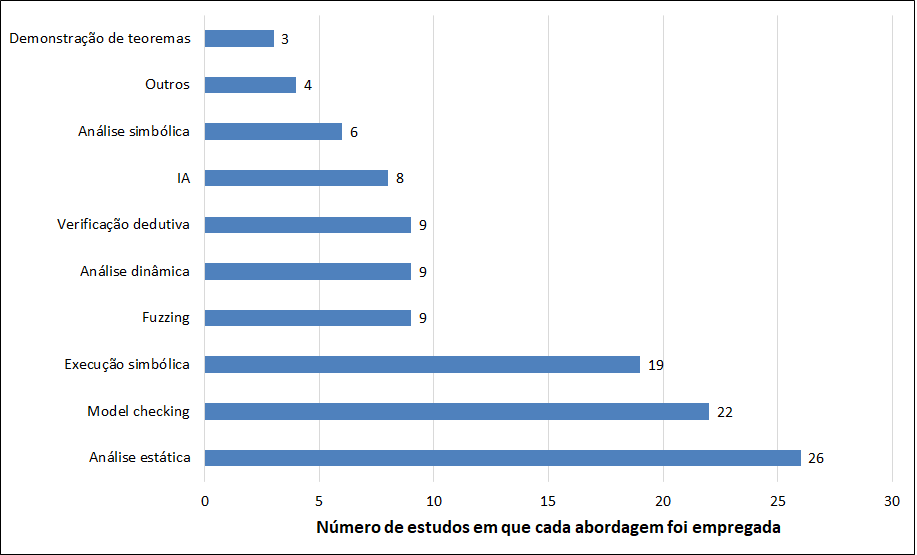
\includegraphics[scale=0.6]{figuras/rq1-abordagens.png}
 \fdadospesquisa
\end{figure}

\begin{table}[!ht]
\centering
\fontsize{8pt}{8pt}\selectfont
\caption{Abordagens híbridas para verificação de CIs}
\label{tab:rq1-hibridas}
\begin{tabular}{@{}ll@{}}
\toprule
\textbf{ID}            & \textbf{Métodos de verificação}               \\ \midrule
\#02, \#07, \#62, \#79 & Análise estática e execução simbólica         \\
\#69, \#76, \#88       & Análise estática e análise dinâmica           \\
\#37                   & Execução simbólica e \textit{fuzzing}                  \\
\#38                   & Execução simbólica e demonstração de teoremas \\
\#64                   & Análise dinâmica e \textit{fuzzing}                    \\
\#90                   & \textit{Fuzzing} e \textit{machine learning}                    \\ \bottomrule
\end{tabular}
\fdadospesquisa
\end{table}

Entre as abordagens baseadas em \textit{model checking} observou-se quatro variações da aplicação desta técnica, consideradas como sub-categorias desta questão de pesquisa. Da mesma forma, também foram identificadas duas sub-categorias entre as abordagens de IA. Os estudos que utilizam \textit{model checking} são expostos na Tabela~\ref{tab:rq1-model-check}. Das abordagens baseadas em IA, em \#08,\#14, \#20, \#54, \#84 e \#90 são aplicadas técnicas de \textit{machine learning}, enquanto que em \#16 e \#96 é utilizado \textit{deep learning}. Dos estudos englobados na categoria \textit{outras}, foram aplicadas as seguintes técnicas de verificação: execução concólica (\#12); refinamento de abstração (\#67); pesquisa genética e teste de mutação (\#83); e interpretação abstrata (\#95).

Quanto ao tipo de verificação houve pouca variação, com 96\% (100 de 104) dos estudos propondo uma estratégia de verificação proativa. A verificação em tempo de execução é pouco explorada, e está presente apenas em \#19, \#30, \#61 e \#77 (4\%). 


\begin{table}[!ht]
\centering
\fontsize{8pt}{8pt}\selectfont
\caption{Técnicas de \textit{model checking} empregadas para verificação de CIs}
\label{tab:rq1-model-check}
\begin{tabular}{@{}ll@{}}
\toprule
\textbf{ID}            & \textbf{Técnica de \textit{model checking} empregada} \\ \midrule
\begin{tabular}[c]{@{}l@{}}\#04, \#10, \#11, \#28, \#40, \#41 \\ \#42, \#45, \#46, \#47, \#58, \#59\\ \#60, \#78, \#101, \#103\end{tabular} & \textit{Model checking} tradicional \\
\#26, \#32, \#48, \#87 & \textit{Model checking} limitado                      \\
\#17, \#22             & \textit{Model checking} simbólico                     \\
\#44                   & \textit{Model checking} estatístico                   \\ \bottomrule
\end{tabular}
\fdadospesquisa
\end{table}
%depois vê se vai considerar uma categoria geral de verificação formal para englobar model checking e verificação dedutiva.

\subsubsection*{\textbf{Classificação das publicações por ano e veículo de publicação (QP 2)}}

Com o propósito de oferecer uma visão geral dos esforços empregados para verificação de CIs, na Figura~\ref{fig:rq2-distribuicao-estudos} é exibido a distribuição dos 104 estudos ao longo dos anos. Como pode-se observar, os esforços para verificação de CIs são recentes, iniciando em 2016 e crescendo rapidamente, principalmente a partir de 2018. Ademais, como complemento à \textbf{QP. 1}, no gráfico da Figura~\ref{fig:rq2-distribuicao-abordagens} é exposto a distribuição da utilização das abordagens para verificação de CIs em cada ano, e na Tabela~\ref{tab:rq2-distribuicao-abordagens} essa distribuição é exibida com a identificação dos estudos. Deste modo, observa-se que análise estática, \textit{model checking} e análise simbólica, além de serem as abordagem mais utilizadas, são as que mais prevaleceram ao longo dos últimos anos. 

\begin{figure}[!htb]
 \caption{Distribuição dos estudos selecionados ao longo dos anos}
 \label{fig:rq2-distribuicao-estudos}
 \centering
 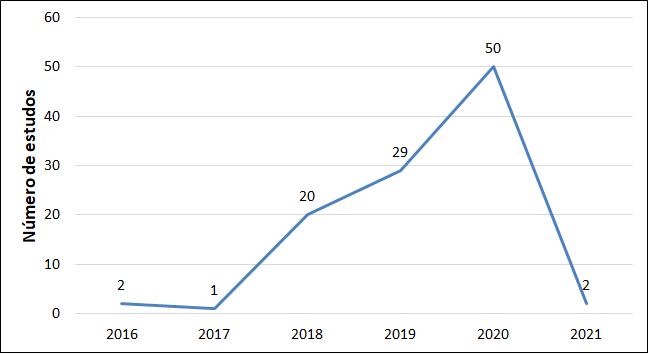
\includegraphics[scale=0.6]{figuras/rq2-distribuicao-estudos.png}
 \fdadospesquisa
\end{figure}

\begin{figure}[!htb]
 \caption{Distribuição das abordagens para verificação de CIs empregadas ao longo dos anos}
 \label{fig:rq2-distribuicao-abordagens}
 \centering
 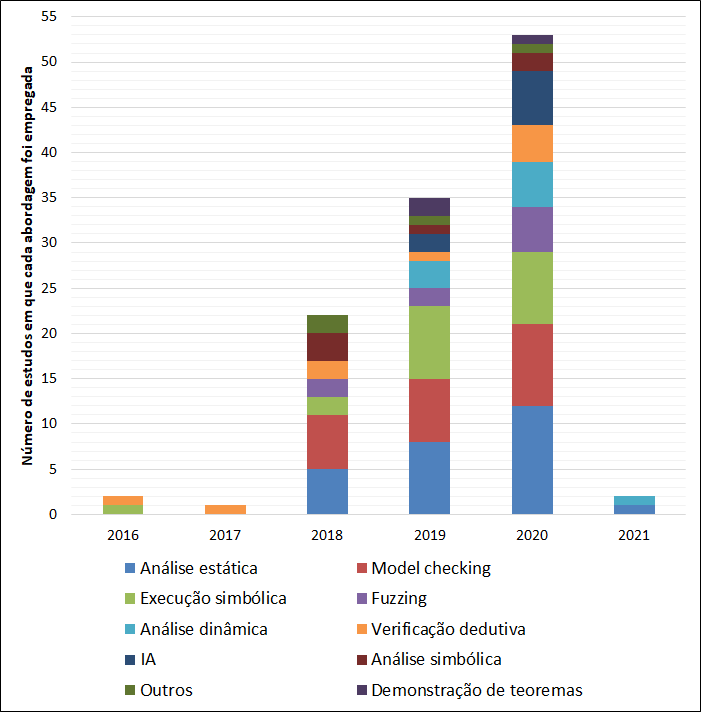
\includegraphics[scale=0.6]{figuras/rq2-distribuicao-abordagens.png}
 \fdadospesquisa
\end{figure}

\begin{table}[!ht]
\centering
\fontsize{8pt}{8pt}\selectfont
\caption{Abordagens para verificação de CIs empregadas ao longo dos anos}
\label{tab:rq2-distribuicao-abordagens}
\begin{tabular}{@{}lllllll@{}}
\toprule
\textbf{Abordagem} &
  \textbf{2016} &
  \textbf{2017} &
  \textbf{2018} &
  \textbf{2019} &
  \textbf{2020} &
  \textbf{2021} \\ \midrule
Análise estática &
   &
   &
  \begin{tabular}[c]{@{}l@{}}\#55, \#76, \#79, \#85\\ \#98\end{tabular} &
  \begin{tabular}[c]{@{}l@{}}\#2, \#62, \#63, \#66\\ \#73, \#80, \#81, \#88\end{tabular} &
  \begin{tabular}[c]{@{}l@{}}\#06, \#07, \#21, \#27\\ \#31, \#34, \#69, \#71\\ \#75, \#77, \#86, \#91\end{tabular} &
  \#29 \\ \midrule
\textit{Model checking} &
   &
   &
  \begin{tabular}[c]{@{}l@{}}\#17, \#41, \#44, \#45\\ \#59, \#87\end{tabular} &
  \begin{tabular}[c]{@{}l@{}}\#22, \#26, \#28, \#42\\ \#46, \#78, \#103\end{tabular} &
  \begin{tabular}[c]{@{}l@{}}\#04, \#10, \#11, \#32\\ \#40, \#48, \#58, \#60\\ \#101\end{tabular} &
   \\ \midrule
Execução simbólica &
  \#56 &
   &
  \#65, \#79 &
  \begin{tabular}[c]{@{}l@{}}\#2, \#36, \#37, \#38\\ \#57, \#62, \#74, \#82\end{tabular} &
  \begin{tabular}[c]{@{}l@{}}\#07, \#13, \#25, \#50\\ \#68, \#89, \#97, \#104\end{tabular} &
   \\ \midrule
\textit{Fuzzing} &
   &
   &
  \#18, \#70 &
  \#37, \#90 &
  \begin{tabular}[c]{@{}l@{}}\#33, \#35, \#51, \#52\\ \#64\end{tabular} &
   \\ \midrule
Análise dinâmica &
   &
   &
   &
  \#30, \#61, \#88 &
  \begin{tabular}[c]{@{}l@{}}\#01, \#19, \#49, \#64\\ \#69\end{tabular} &
  \#53 \\ \midrule
Verificação dedutiva &
  \#47 &
  \#24 &
  \#5, \#99 &
  \#100 &
  \#09, \#15, \#23, \#102 &
   \\ \midrule
IA &
   &
   &
   &
  \#54, \#90 &
  \begin{tabular}[c]{@{}l@{}}\#08, \#14, \#16, \#20\\ \#84, \#96\end{tabular} &
   \\ \midrule
Análise simbólica &
   &
   &
  \#39, \#76, \#93 &
  \#94 &
  \#72, \#92 &
   \\ \midrule
Outras &
   &
   &
  \#67, \#95 &
  \#12 &
  \#83 &
   \\ \midrule
Demonstração de teoremas &
   &
   &
   &
  \#38, \#43 &
  \#03 &
   \\ \bottomrule
\end{tabular}
\fdadospesquisa
\end{table}

Os estudos selecionados foram publicados em Conferências, Periódicos e Workshops. Conferências têm sido o principal veículo de publicação, abrangendo 73\% (76 de 104 estudos). Em seguida, os estudos publicados em Periódicos representam 22\% (23 de 104). Por fim, apenas 5 estudos foram apresentados em Workshops (5\%). Constata-se que, apesar da maioria dos estudos terem sido publicados em conferências, não há um meio de publicação padrão para este tipo de pesquisa, assim como os eventos e periódicos de publicação, que também são variados.

%fazer tabela com cada evento/periódico de cada estudo????

\subsubsection*{\textbf{Vulnerabilidades e problemas tratados pelas abordagens de verificação de CIs (QP 3)}}

%DEPOIS TEM QUE GERAR DE NOVO O GRÁFICO DAS VULNERABILIDADES

Na Figura~\ref{fig:rq3-vulnerabilidades} é exibido um gráfico que ilustra o número de estudos em que cada vulnerabilidade e problema é tratado. Desta forma, pode-se notar o foco dos esforços despendidos para verificação de CIs, principalmente para as vulnerabilidades de reentrância $V_{23}$, \textit{integer overflow} e \textit{underflow} $V_{20}$, exceções não tratadas $V_{18}$ e dependência de \textit{timestamp}$V_{14}$, e também para a detecção de violação de propriedades ($VP$). Os estudos em que cada um dos itens são abordados são listados na Tabela~\ref{tab:rq3-estudos-vulnerabilidades}.

\begin{figure}[!htb]
 \caption{Distribuição das vulnerabilidades e problemas tratados na verificação de CIs}
 \label{fig:rq3-vulnerabilidades}
 \centering
 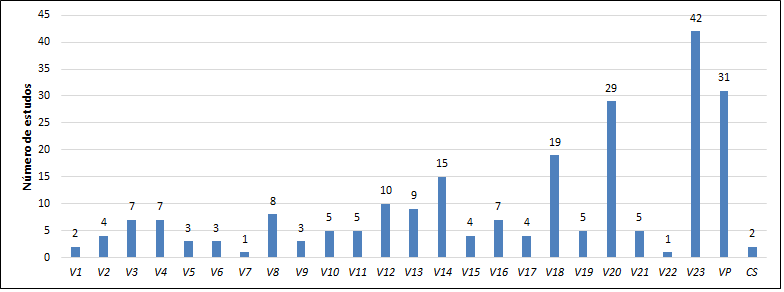
\includegraphics[scale=0.7]{figuras/rq3-vulnerabilidades.png}
 \fdadospesquisa
\end{figure}

\begin{table}[!ht]
\centering
\fontsize{8pt}{8pt}\selectfont
\caption{Estudos que abordam cada uma das vulnerabilidades e problemas dos CIs}
\label{tab:rq3-estudos-vulnerabilidades}
\begin{tabular}{@{}clcl@{}}
\toprule
\multicolumn{1}{l}{\textbf{\begin{tabular}[c]{@{}l@{}}Vulnerabilidade/\\ Problema\end{tabular}}} &
  \textbf{Estudos} &
  \multicolumn{1}{l}{\textbf{\begin{tabular}[c]{@{}l@{}}Vulnerabilidade/\\ Problema\end{tabular}}} &
  \textbf{Estudos} \\ \midrule
$V_{1}$ &
  \#20, \#79 &
  $V_{14}$ &
  \begin{tabular}[c]{@{}l@{}}\#14, \#16, \#18, \#20, \#26, \#51, \#56, \#71\\ \#79, \#82, \#84, \#85, \#88, \#90, \#92\end{tabular} \\ \midrule
$V_{2}$ &
  \#33, \#75, \#84, \#90 &
  $V_{15}$ &
  \#18, \#51, \#64, \#83 \\ \midrule
$V_{3}$ &
  \#19, \#27, \#63, \#71, \#79, \#85, \#88 &
  $V_{16}$ &
  \#65, \#79, \#80, \#85, \#87, \#88, \#102 \\ \midrule
$V_{4}$ &
  \#18, \#28, \#33, \#63, \#81, \#85, \#101 &
  $V_{17}$ &
  \#08, \#33, \#90, \#101 \\ \midrule
$V_{5}$ &
  \#50, \#63, \#98 &
  $V_{18}$ &
  \begin{tabular}[c]{@{}l@{}}\#02, \#07, \#13, \#18, \#19, \#33, \#35, \#36\\ \#47, \#51, \#53, \#56, \#63, \#76, \#81, \#85\\ \#88, \#92, \#101\end{tabular} \\ \midrule
$V_{6}$ &
  \#08, \#13, \#39 &
  $V_{19}$ &
  \#26, \#63, \#86, \#90, \#101 \\ \midrule
$V_{7}$ &
  \#39 &
  $V_{20}$ &
  \begin{tabular}[c]{@{}l@{}}\#02, \#03, \#05, \#07, \#08, \#14, \#16, \#19\\ \#20, \#30, \#33, \#52, \#53, \#55, \#63, \#56\\ \#65, \#71, \#75, \#80, \#83, \#86, \#87, \#88\\ \#89, \#90, \#91, \#92, \#102\end{tabular} \\ \midrule
$V_{8}$ &
  \#02, \#31, \#32, \#39, \#62, \#71, \#81, \#101 &
  $V_{21}$ &
  \#16, \#17, \#29, \#55, \#98 \\ \midrule
$V_{9}$ &
  \#16, \#53, \#94 &
  $V_{22}$ &
  \#45 \\ \midrule
$V_{10}$ &
  \#35, \#53, \#63, \#75, \#90 &
  $V_{23}$ &
  \begin{tabular}[c]{@{}l@{}}\#01, \#02, \#04, \#06, \#14, \#16, \#18, \#19\\ \#20, \#21, \#24, \#26, \#27, \#33, \#34, \#37\\ \#47, \#51, \#52, \#53, \#56, \#62, \#63, \#64\\ \#68, \#69, \#70, \#71, \#75, \#76, \#79, \#81\\ \#82, \#83, \#84, \#85, \#86, \#89, \#90, \#92\\ \#96, \#101\end{tabular} \\ \midrule
$V_{11}$ &
  \#02, \#13, \#18, \#19, \#31 &
  $VP$ &
  \begin{tabular}[c]{@{}l@{}}\#07, \#09, \#10, \#11, \#15, \#21, \#22, \#23, \#24\\ \#28, \#34, \#40, \#41, \#42, \#43, \#44, \#46\\ \#47, \#58, \#59, \#60, \#61, \#73, \#74, \#77\\ \#78, \#89, \#97, \#99, \#100, \#103, \#104\end{tabular} \\ \midrule
$V_{12}$ &
  \begin{tabular}[c]{@{}l@{}}\#02, \#13, \#18, \#33, \#51, \#53, \#63, \#75\\ \#90, \#92\end{tabular} &
  $CSS$ &
  \#07, \#48 \\ \midrule
$V_{13}$ &
  \begin{tabular}[c]{@{}l@{}}\#02, \#20, \#26, \#37, \#56, \#76, \#79, \#83\\ \#90\end{tabular} &
   &
   \\ \bottomrule
\end{tabular}
\end{table}

\subsubsection*{\textbf{Estratégias de validação utilizadas (\textbf{QP 4})}}

Dos 104 estudos selecionados, em 76 (73\%) o método de verificação proposto é implementado por meio de um framework ou ferramenta (\textit{M1}), e em 22 (21\%) é utilizado um framework ou ferramenta já existente (\textit{M2}). Nos outros 6 estudos (6\%) a verificação é descrita como um processo (\textit{M3}), e, portanto, não é retratado o desenvolvimento ou o uso de algum \textit{software} para guiar ou automatizar o procedimento de verificação. Conforme ilustrado no gráfico da Figura~\ref{fig:rq4-aplicacao-propostas} a utilização de um dos mecanismos de aplicação das propostas pode variar de acordo a abordagem de verificação. Na maior parte das abordagens de verificação baseadas em \textit{fuzzing} (8 dos 9 estudos), demonstração de teoremas (2 dos 3), execução simbólica (18 dos 19) e análise estática (25 dos 26), foram implementados frameworks ou ferramentas de verificação. A utilização de frameworks ou ferramentas já existentes prevaleceu principalmente nas categorias de verificação dedutiva e \textit{model checking} (5 dos 9, e 14 dos 22 estudos, respectivamente). A aplicação da verificação como descrição de um processo ocorreu apenas em uma das propostas de verificação dedutiva e \textit{fuzzing}, e também em 5 das 8 propostas baseadas em IA. Por fim, nas categorias de análise simbólica, análise dinâmica e em outras, todos os estudos empregam o mecanismo \textit{M1}.   

\begin{figure}[!htb]
 \caption{Utilização dos mecanismos de aplicação das propostas em cada abordagem de verificação}
 \label{fig:rq4-aplicacao-propostas}
 \centering
 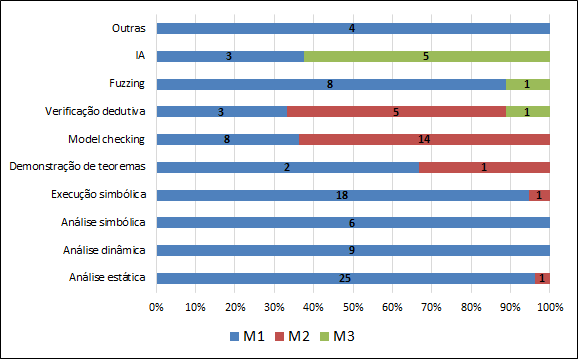
\includegraphics[scale=0.7]{figuras/rq4-aplicacao-propostas.png}
 \fdadospesquisa
\end{figure}

Entre as estratégias de validação das propostas, em 63\% dos estudos foi aplicado algum experimento, enquanto que o estudo de caso e o exemplo de aplicação foram utilizados como prova de conceito em 25\% e 14\% dos estudos, respectivamente. Na Figura~\ref{fig:rq4-validacao-propostas} é mostrada a frequência em as estratégias de validação são empregadas sobre cada uma das abordagens de verificação. Assim, nota-se uma quantidade relativamente baixa de experimentos nas propostas de verificação dedutiva e \textit{model checking}, enquanto que na demonstração de teoremas nenhum experimento foi executado.

\begin{figure}[!htb]
 \caption{Utilização das estratégias de validação em cada abordagem de verificação}
 \label{fig:rq4-validacao-propostas}
 \centering
 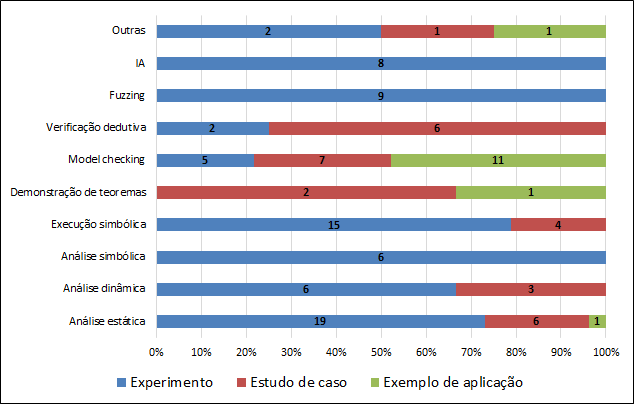
\includegraphics[scale=0.65]{figuras/rq4-validacao-propostas.png}
 \fdadospesquisa
\end{figure}

No total, 65 dos 104 estudos realizaram algum experimento para validação das propostas, e, dentre esses, um ou mais procedimentos foram aplicados ao longo do processo de experimentação. Dos 65 estudos, em 47 (72\%) é aplicado um experimento em larga escala, enquanto que em 38 (37\%) é realizado um experimento reduzido e em 28 (43\%) é acrescentado algum procedimento para avaliação empírica. A relação do número de estudos nos quais foram descritos ao menos um dos procedimentos experimentais citados é ilustrada no diagrama de Venn Figura~\ref{fig:rq4-diagrama-experimento}. Vale salientar que, os números 14 e 18, que estão fora das intersecções, representam o número de estudos nos quais foi aplicado apenas o procedimento de experimento reduzido ou em larga escala, nesta ordem.

\begin{figure}[!htb]
 \caption{Procedimentos aplicados sobre os estudos que realizaram validação experimental}
 \label{fig:rq4-diagrama-experimento}
 \centering
 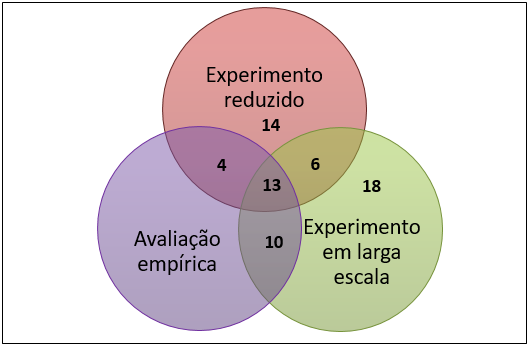
\includegraphics[scale=0.7]{figuras/rq4-diagrama-experimento.png}
 \fdadospesquisa
\end{figure}

% inserir tabelas com a identificação dos estudos de cada gráfico????

\subsubsection*{Limitações presentes nas abordagens (\textbf{QP 5})}

%falar das limitações dos tipo em tempo de execução e CBC

Em relação à abrangência da verificação de CIs, em 70\% (73 de 104) dos estudos o método empregado engloba todos elementos da linguagem Solidity, ou outra linguagem para programação de CIs considerada, enquanto no restante (31 de 104) é considerado apenas algum subconjunto de elementos da linguagem. Quanto ao nível de automatização, em 66\% (69 de 104) dos estudos é proposta uma estratégia automática para verificação, enquanto em 9\% (9) a verificação é feita manualmente, ou então não é descrito nenhum mecanismo de automatização. Os outros 26 estudos (25\%) empregam estratégias semi-automatizadas, das quais é necessário execução manual de ao menos um dos seguintes procedimentos: (i) tradução de código (9); obtenção do modelo a ser verificado (16); especificação das propriedades (22); e análise e interpretação dos resultados (9). Informações sobre a abrangência e o nível de automação de cada abordagem de verificação são expostas nas Figuras~\ref{fig:rq5-abrangencia} e ~\ref{fig:rq5-automacao}, respectivamente, e os estudos incluídos em cada uma das classificações são listados nas Tabelas~\ref{tab:rq5-limitacoes} e~\ref{tab:rq5-procedimentos-manuais}. 

\begin{figure}[!htb]
 \caption{Abrangência das abordagem para verificação de CIs}
 \label{fig:rq5-abrangencia}
 \centering
 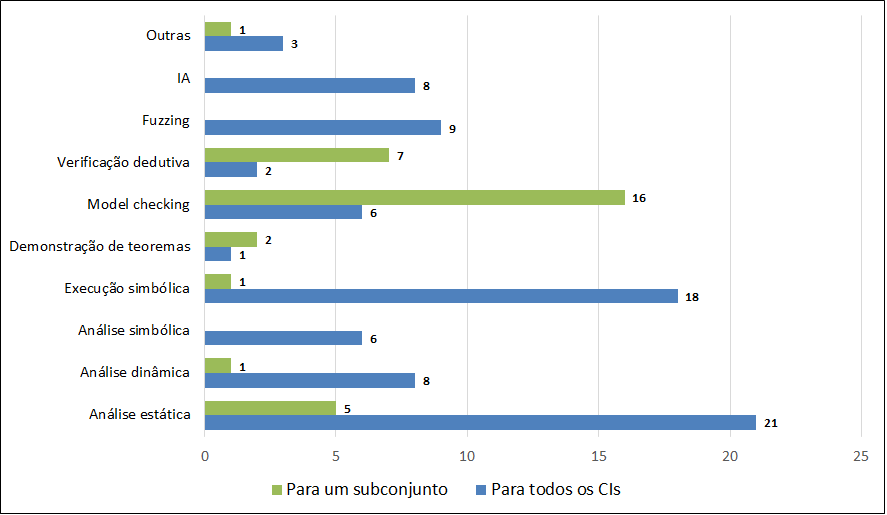
\includegraphics[scale=0.6]{figuras/rq5-abrangencia.png}
 \fdadospesquisa
\end{figure}

\begin{figure}[!htb]
 \caption{Nível de automação das abordagem para verificação de CIs}
 \label{fig:rq5-automacao}
 \centering
 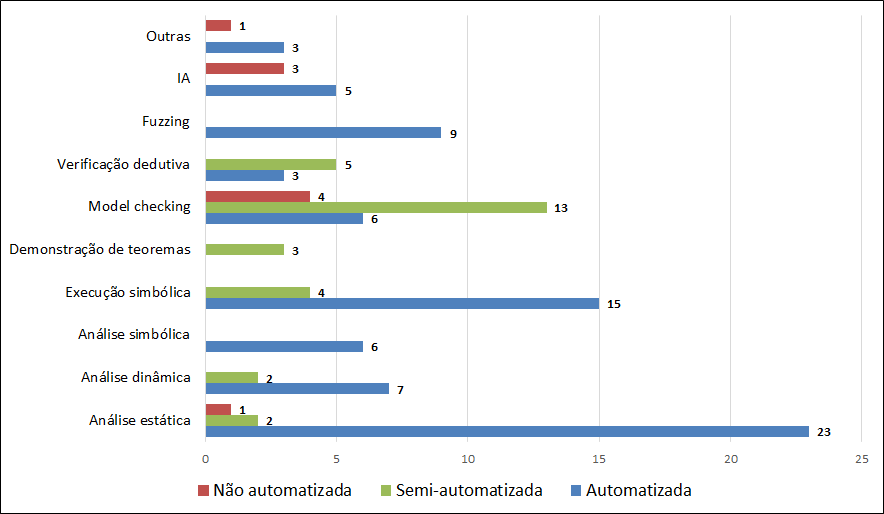
\includegraphics[scale=0.6]{figuras/rq5-automacao.png}
 \fdadospesquisa
\end{figure}

\begin{table}[!ht]
\centering\fontsize{8pt}{8pt}\selectfont
\caption{Abrangência e automação das abordagens de verificação de CIs}
\label{tab:rq5-limitacoes}
\begin{tabular}{l|ll|lll}
\multirow{\textbf{Abordagem}} &
  \multicolumn{2}{c|}{\textbf{Abrangência}} &
  \multicolumn{3}{c}{\textbf{Automação}} \\
 &
  \textbf{Para todos os CIs} &
  \textbf{Para um subconjunto} &
  \textbf{Automatizada} &
  \textbf{Semi-Automatizada} &
  \textbf{Não automatizada} \\ \hline
\textbf{\begin{tabular}[c]{@{}l@{}}Análise \\ estática\end{tabular}} &
  \begin{tabular}[c]{@{}l@{}}\#02, \#21, \#27, \#29, \#31\\ \#34, \#55, \#62, \#63, \#71\\ \#75, \#76, \#77, \#79, \#80\\ \#81, \#85, \#86, \#88, \#91\\ \#98\end{tabular} &
  \#06, \#07, \#66, \#69, \#73 &
  \begin{tabular}[c]{@{}l@{}}\#02, \#21, \#27, \#29, \#31\\ \#34, \#55, \#62, \#63, \#66\\ \#71, \#73, \#75, \#76, \#77\\ \#79, \#80, \#81, \#85, \#86\\ \#88, \#91, \#98\end{tabular} &
  \#07, \#69 &
  \#06 \\ \hline
\textbf{\begin{tabular}[c]{@{}l@{}}Análise \\ dinâmica\end{tabular}} &
  \begin{tabular}[c]{@{}l@{}}\#39, \#72, \#76, \#92, \#93\\ \#94\end{tabular} &
   &
  \begin{tabular}[c]{@{}l@{}}\#39, \#72, \#76, \#92, \#93\\ \#94\end{tabular} &
   &
   \\ \hline
\textbf{\begin{tabular}[c]{@{}l@{}}Análise \\ simbólica\end{tabular}} &
  \begin{tabular}[c]{@{}l@{}}\#39, \#72, \#76, \#92, \#93\\ \#94\end{tabular} &
   &
  \begin{tabular}[c]{@{}l@{}}\#39, \#72, \#76, \#92, \#93\\ \#94\end{tabular} &
   &
   \\ \hline
\textbf{\begin{tabular}[c]{@{}l@{}}Execução \\ simbólica\end{tabular}} &
  \begin{tabular}[c]{@{}l@{}}\#02, \#13, \#25, \#36, \#37\\ \#38, \#50, \#56, \#57, \#62\\ \#65, \#68, \#74, \#79, \#82\\ \#89, \#97, \#104\end{tabular} &
  \#7 &
  \begin{tabular}[c]{@{}l@{}}\#02, \#13, \#25, \#36, \#37\\ \#50, \#56, \#57, \#62, \#65\\ \#68, \#74, \#79, \#82, \#89\end{tabular} &
  \#7, \#38, \#97, \#104 &
   \\ \hline
\textbf{\begin{tabular}[c]{@{}l@{}}Demonstração \\ de teoremas\end{tabular}} &
  \#38 &
  \#03, \#43 &
   &
  \#03, \#38, \#43 &
   \\ \hline
\textbf{\begin{tabular}[c]{@{}l@{}}Model \\ checking\end{tabular}} &
  \begin{tabular}[c]{@{}l@{}}\#10, \#26, \#32, \#48, \#101\\ \#103\end{tabular} &
  \begin{tabular}[c]{@{}l@{}}\#04, \#11, \#17, \#22, \#28\\ \#40, \#41, \#42, \#44, \#45\\ \#46, \#47, \#58, \#59, \#60\\ \#78, \#87\end{tabular} &
  \begin{tabular}[c]{@{}l@{}}\#10, \#26, \#32, \#47, \#48\\ \#87\end{tabular} &
  \begin{tabular}[c]{@{}l@{}}\#04, \#11, \#22, \#28, \#41\\ \#44, \#45, \#46, \#58, \#59\\ \#78, \#101, \#103\end{tabular} &
  \#17, \#40, \#42, \#60 \\ \hline
\textbf{\begin{tabular}[c]{@{}l@{}}Verificação \\ dedutiva\end{tabular}} &
  \#100, \#102 &
  \begin{tabular}[c]{@{}l@{}}\#05, \#09, \#15, \#23, \#24\\ \#99\end{tabular} &
  \#15, \#23, \#102 &
  \#05, \#09, \#24, \#99, \#100 &
   \\ \hline
\textbf{Fuzzing} &
  \begin{tabular}[c]{@{}l@{}}\#18, \#33, \#35, \#37, \#51\\ \#52, \#64, \#70, \#90\end{tabular} &
   &
  \begin{tabular}[c]{@{}l@{}}\#18, \#33, \#35, \#37, \#51\\ \#52, \#64, \#70, \#90\end{tabular} &
   &
   \\ \hline
\textbf{IA} &
  \begin{tabular}[c]{@{}l@{}}\#08, \#14, \#20, \#54, \#84\\ \#90, \#16, \#96\end{tabular} &
   &
  \#20, \#84, \#90, \#16, \#96 &
   &
  \#08, \#14, \#54 \\ \hline
\textbf{Outras} &
  \#12, \#83, \#95 &
  \#67 &
  \#12, \#83,   \#95 &
   &
  \#67 \\ \hline
\end{tabular}
\fdadospesquisa
\end{table}

\begin{table}[!ht]
\centering
\fontsize{8pt}{8pt}\selectfont
\caption{Procedimentos manuais realizados nos métodos semi-automatizados}
\label{tab:rq5-procedimentos-manuais}
\begin{tabular}{l|llll}
\multirow{\textbf{Abordagem}}                                          & \multicolumn{4}{c}{\textbf{Procedimentos manuais}}                  \\
 &
  \textbf{Tradução de código} &
  \textbf{Obtenção do modelo} &
  \textbf{\begin{tabular}[c]{@{}l@{}}Especificação das \\ propriedades\end{tabular}} &
  \textbf{\begin{tabular}[c]{@{}l@{}}Análise e interpretação\\ dos resultados\end{tabular}} \\ \hline
\textbf{\begin{tabular}[c]{@{}l@{}}Análise \\ estática\end{tabular}}         & \#69       &                  & \#07                    &            \\ \hline
\textbf{\begin{tabular}[c]{@{}l@{}}Execução \\ simbólica\end{tabular}}       & \#97       &                  & \#07, \#38, \#97, \#104 & \#38       \\ \hline
\textbf{\begin{tabular}[c]{@{}l@{}}Demonstração \\ de teoremas\end{tabular}} &            & \#03, \#43       & \#38, \#43              & \#38, \#43 \\ \hline
\textbf{\begin{tabular}[c]{@{}l@{}}Model \\ checking\end{tabular}} &
  \#11, \#22, \#45, \#59, \#78 &
  \begin{tabular}[c]{@{}l@{}}\#11, \#22, \#41, \#44, \#45\\ \#46, \#58, \#59, \#78, \#101\\ \#103\end{tabular} &
  \begin{tabular}[c]{@{}l@{}}\#11, \#22, \#28, \#41, \#44\\ \#45, \#46, \#58, \#59, \#78\\ \#101, \#103\end{tabular} &
  \begin{tabular}[c]{@{}l@{}}\#04, \#41, \#44, \#45, \#46\\ \#78\end{tabular} \\ \hline
\textbf{\begin{tabular}[c]{@{}l@{}}Verificação \\ dedutiva\end{tabular}}     & \#24, \#99 & \#05, \#24, \#99 & \#05, \#24, \#99, \#100 & \#09       \\ \hline
\end{tabular}
\fdadospesquisa
\end{table}

Das abordagens de verificação, as únicas nas quais a maioria dos trabalhos não abrange todos os elementos dos CIs foram o \textit{model checking} (16 entre 22 estudos), a verificação dedutiva (7 entre 9) e a demonstração de teoremas (2 entre 3). Já na análise estática, análise dinâmica, execução simbólica, e em Outras, na vasta maioria dos estudos todos os aspectos dos CIs são aceitos para verificação, enquanto que na análise simbólica, \textit{fuzzing}, e IA isso se enquadra à todos os trabalhos selecionados. 

Quanto ao nível de automação, nota-se que há poucos (ou nenhum) trabalhos semi ou não automatizados entre as abordagens de análise estática, análise dinâmica, análise simbólica, \textit{fuzzing}, e em Outras. Dentre os estudos focados em IA, 3 das 8 propostas foram classificadas como não automatizadas, pois não foram fornecidas informações suficientes para concluir que a verificação é feita de forma automática. Entre as propostas de demonstração de teoremas, \textit{model checking} e verificação dedutiva, todas, ou a maioria não são automatizadas.

Com exceção da demonstração de teoremas, do \textit{model checking} e da verificação dedutiva, foi observada a ocorrência de falsos positivos e falsos negativos entre as vulnerabilidades detectadas pelas ferramentas e frameworks implementados, principalmente quando utilizadas técnicas de análise estática e execução simbólica. De forma indireta, este problema atingiu também os estudos baseados em IA, já que, em alguns destes (\#20, \#54 e \#90), os modelos utilizados para treinamento dos algoritmos de detecção são criados a partir dos resultados obtidos de ferramentas que apresentam altas taxas de falsos positivos e falsos negativos, o que pode ter influenciado a qualidade dos modelos. A ocorrência de falsos positivos e falsos negativos foi notada também em técnicas de análise dinâmica, análise simbólica e \textit{fuzzing}.

As abordagens de demonstração de teoremas, \textit{model checking} e verificação dedutiva destacam-se pela sua precisão, já que não produzem falsos positivos e negativos. Porém, estas baseiam-se na aplicação de métodos formais, e exigem algum conhecimento específico sobre técnicas de modelagem e verificação de propriedades, que geralmente não são dominadas por desenvolvedores.  

\subsection{Discussão} \label{tex:rev:ms:discussao}

Plataformas blockchain baseadas na execução de CIs, como a Ethereum, têm ganhado notável destaque e popularidade nos últimos anos, e foram aplicadas em diversas áreas. Por outro lado, houve também ataques sobre diversos CIs nos quais usuários maliciosos de aproveitaram de vulnerabilidades de segurança presentes nos códigos dos CIs para transferir para a própria conta o Ether associado ao contrato. Estes ataques mobilizaram a academia e a indústria, e, nos últimos ano houve um aumento expressivo das pesquisas que buscam mitigar os riscos destas vulnerabilidades, que iniciaram-se em 2016. Assim, a verificação e detecção de vulnerabilidades em CIs é um tópico de pesquisa recente e diversas abordagens distintas têm sido empregadas. A identificação e classificação dessas abordagens foi o foco desse MS, que também apontou a frequência da utilização dessas abordagens ao longo dos anos, as vulnerabilidades e problemas alvos de verificação, as estratégias de validação empregadas e as principais limitações presentes nestes trabalhos.

Entre os 104 estudos selecionados, as abordagens de verificação mais utilizada, e que também foram as que mais prevaleceram ao longo dos anos foram as baseadas em execução simbólica, \textit{model checking}, e análise estática. Foram classificados neste MS 25 problemas e vulnerabilidades alvos de verificação. Destes, nota-se que a Reentrância ($V_{23}$) foi a vulnerabilidade mais investigada pelos estudos, o que provavelmente deve-se ao fato desta ter sido a primeira a ser explorada, o que resultou no ataque ao contrato \textit{The DAO} e mobilizou a comunidade em torno deste problema. 

Uma forma mais genérica de verificar se a execução de um contrato é realizada conforme esperado é por meio da verificação da violação de propriedades ($VP$), as quais podem estar relacionadas com problemas de segurança, e também com o cumprimento de requisitos de projeto, funcionais, e lógicos. As propriedades são definidas especialmente para cada contrato, um trabalho manual que exige um alto nível de compreensão dos requisitos do contrato, assim como o conhecimento específico do formalismo ou linguagem de especificação utilizado. A violação de propriedades têm sido tratada principalmente pelas abordagens baseadas em \textit{model checking} (em 15 estudos).

Outra questão analisada neste MS foram as estratégias da validação utilizada nos estudos (\textbf{QP 4}). Desta forma pôde-se observar desde estratégias simples e triviais como exemplos de aplicação e estudos de caso, até as mais robustas, compostas por vários procedimentos experimentais. Em muitos casos, devido a falta de uma validação mais completa e robusta, não foi possível tirar conclusões sobre questões como a eficiência e acurácia dos métodos propostos (como nos estudos \#11, \#15, \#22, \#23, \#27, \#58, \#59, \#60, \#69, \#70, \#71, \#75, \#78, \#82, \#87, \#95, \#98, \#100 e \#103).  

Ao longo dos resultados da \textbf{QP 5}, a abordagens foram classificadas em relação à abrangência da verificação e ao nível de automação da estratégia empregada, o que envolve não apenas a verificação em si, mas também procedimentos aplicados antes e após. Apenas no \textit{model checking}, na demonstração de teoremas, e na verificação dedutiva, os métodos propostos nos estudos foram majoritariamente aplicados apenas sobre um subconjunto da linguagem de programação de CIs considerada, o que indica necessidade de avanços nessa área para expandir a verificação sobre mais elementos dos CIs e abranger contratos mais complexos e variados. Também, nestas três abordagens, notou-se, na maior parte dos estudos, a aplicação de procedimentos manuais ao longo da estratégia de verificação. Entretanto, o fato de um método não ser totalmente automatizado não representa, necessariamente, uma desvantagem, pois depende do fim para o qual ele é proposto. Por exemplo, em muitos casos pode ser desejável que propriedades sejam definidas manualmente, pois cada contrato possui requisitos específicos relacionados ao seu projeto e seu propósito.

De forma geral, ainda não há uma convergência ou consenso sobre qual método de verificação é o melhor, pois ainda é uma área de estudo recente, e várias abordagens mostram-se promissoras, tantos aquelas utilizadas a mais tempo quantos a mais recentes, como as baseadas em IA. Contudo, ainda há diversas limitações presentes, que servirão de motivação das pesquisas e avanços futuros nesta área.

% ferramentas de model checking não funcionam para todos os elementos da linguagem, porém, elas tem o intuito de abordar propriedades específicas. MC é um método custoso, e quando aplicado, não costuma ser para todo o sistema, mas apenas para uma parte mais crítica \cite{peled2019formal-methods}
\section{Seleção dos fundamentos da proposta}

A realização do MS descrito na Seção~\ref{tex:rev:ms} constituiu a primeira das quatro tarefas de pesquisa descritas no início deste Capítulo, e serve de base para a execução das próximas, que são: 2. Seleção do método de verificação e detecção de vulnerabilidades adequado para a proposta; 3. Seleção das vulnerabilidades abordadas por meio da proposta; e 4. Definição da estratégia para validação da proposta.

O método de verificação escolhido foi o \textit{model checking}, pois há diversos trabalhos na literatura que utilizam esta técnica para verificação de vulnerabilidades de reentrância e para detecção de violação de propriedades. Desta forma, pretende-se focar em vulnerabilidades já conhecidas e também permitir a análise de propriedades funcionais de cada contrato individualmente. Além disso, das abordagens mais utilizadas, o \textit{model checking} apresenta a melhor precisão, com raros casos de falsos positivos e falsos negativos (detectados apenas no estudo \#26).

Das vulnerabilidades abordadas no MS, três foram selecionadas para serem o foco do método de verificação proposto, são elas: reentrância ($V_{23}$); \textit{delegatecall injection} ($V_{13}$); e contrato suicida ($V_{8}$). A primeira foi explorada no \textit{The DAO Attack}, e as outras duas nos ataques cometidos contra o contrato da \textit{Parity Wallet}, ambos citados na Seção~\ref{tex:fund:ethereum:vuln-ataques}. Enquanto a $V_{8}$ e a $V_{23}$ foram abordadas em alguns trabalhos que empregam o \textit{model checking}~\cite{ frank2020ethbmc-32, nelaturu2020verified-101, wang2020formal-04, wang2019detecting-nondeterministic-26}, a $V_{13}$ ainda não foi tratada por meio desta técnica, o que seria um avanço no estado da arte. Como estratégia de validação, pretende-se aplicar um experimento reduzido, com contratos cujas vulnerabilidades já são conhecidas, permitindo, assim, mensurar o nível de acurácia do método. Além disso, também deve ser aplicado um estudo de caso para verificação de violação de propriedades. Demais detalhes sobre o método proposto são descritos adiante no Capítulo~\ref{cap:proposta}.